\documentclass[12pt,a4paper]{report}
\usepackage[margin=3cm]{geometry}
\usepackage{ngerman}
\usepackage{float} 
\usepackage[utf8]{inputenc}
\usepackage[onehalfspacing]{setspace}
\usepackage[numbers,round]{natbib}
\usepackage{graphicx}
\usepackage[colorlinks,
pdfpagelabels,
pdfstartview = FitH,
bookmarksopen = true,
bookmarksnumbered = true,
linkcolor = black,
plainpages = false,
hypertexnames = false,
citecolor = black] {hyperref}


\begin{document}


\pagenumbering{roman}
\thispagestyle{empty}
\begin{verbatim}





\end{verbatim}
\begin{center}
\textbf{\huge{Semantische Beziehungen in Texten mit Word2Vec }}\\
\begin{verbatim}
\end{verbatim}
\textbf{\large{und der Vergleich zwischen allgemeinen und domänenspezifischen Korpora als Trainingsdaten}}
\end{center}
\begin{verbatim}



\end{verbatim}
\begin{center}
\large B A C H E L O R A R B E I T

\begin{verbatim}
\end{verbatim}

\end{center}
\begin{center}
im Studiengang\\
\textsc{Medieninformatik (MI7)}\\
an der Hochschule der Medien in Stuttgart\\
vorgelegt von \textsc{Ruben Müller}\\
\begin{verbatim}
\end{verbatim}
im Juli 2015


\end{center}
\begin{verbatim}







\end{verbatim}

\begin{flushleft}
\begin{tabular}{lll}
\textbf{Erstprüfer:} & & \textsc{Prof. Dr-Ing. Johannes Maucher},\\ 
&&\small Hochschule der Medien, Stuttgart  \\
\textbf{Zweitprüfer:} & & \textsc{M.Sc. Andreas Stiegler},\\
&&\small Hochschule der Medien, Stuttgart\\
\end{tabular}
\end{flushleft}

\newpage
\chapter*{Erklärung}
Hiermit versichere ich, Ruben Müller, an Eides Statt, dass ich die vorliegende
Bachelorarbeit mit dem Titel: \glqq Semantische Beziehungen in Texten mit Word2Vec\grqq{} selbständig und ohne fremde Hilfe verfasst und keine anderen als die angegebenen
Hilfsmittel benutzt habe. Die Stellen der Arbeit, die dem Wortlaut oder dem Sinn nach anderen
Werken entnommen wurden, sind in jedem Fall unter Angabe der Quelle kenntlich gemacht. Die
Arbeit ist noch nicht veröffentlicht oder in anderer Form als Prüfungsleistung vorgelegt worden.\\
Ich habe die Bedeutung der eidesstattlichen Versicherung und die prüfungsrechtlichen Folgen (§ 23 Abs. 2 Bachelor-SPO (7 Semester) der HdM) sowie die strafrechtlichen Folgen (gem. § 156 StGB) einer unrichtigen oder
unvollständigen eidesstattlichen Versicherung zur Kenntnis genommen.\\
\vspace{1em}\\
Filderstadt, den 15. Juli 2015\\
\vspace{5em}\\
Ruben Müller


\newpage
\chapter*{Kurzfassung}
Diese Bachelorarbeit beschäftigt sich mit der Analyse von semantischen Beziehungen innerhalb mit Word2Vec gelernten Modellen.
\\Dazu sollen zum einen der allgemeine komplette Wikipedia-Korpus gelernt und analysiert werden, was als semantisch ähnlich erkannt wird. Zum anderen soll ein Korpus über eine spezielle Domäne erstellt und gelernt werden. Welche spezielle Domäne analysiert und verglichen werden soll, wird im Laufe der Bearbeitung festgelegt.
\\Diese beiden Korpora sollen sich dann gegenüber gestellt und analysiert werden, was jeweils als semantisch ähnlich erkannt wird. 
\\Ziel dieser Arbeit soll es sein, festzustellen ob ein allgemeiner Korpus oder ein spezieller Domänenkorpus genauere Resultate im Hinblick auf semantische Ähnlichkeiten erzielt. Anstatt eines allgemeinen Korpus zu verwenden, könnte es sich dann anbieten zwischen mehreren speziellen Korpora auszuwählen, je nachdem welche Domäne aktuell bearbeitet werden soll.
\newpage
\chapter*{Abstract}
This bachelor thesis deals with the analysis of semantic relations in models which are learnd by Word2Vec.\\
For this purpose on the one hand the whole and general wikipedia body shall be learned and analyzed what is detected as semantic similar. On the other hand a body covering a specific domain shall be created and learned. Which specific domain is choosen will be defined due to the working process.\\
These both bodys shall then be compared against each other to determine what is recognized as semanic similar.\\
Goal of this thesis will be to determine whether a general body or a domain specific body gives more precise results with regard to semantic similarity. Instead of using a general body it coud be better to choose between multiple domain specific bodys with regard to the actual domain.

\newpage
\tableofcontents
\newpage
\chapter*{Begriffsverzeichnis}
	\begin{tabular}{r|l}	
	\textbf{Begriff} & Erklärung\\
	\hline	
	\textbf{Ähnliche Worte} & Im Word2Vec-Modell, mit der Methode\\
	& \textit{most\_similar()}, erhaltene Worte.\\
	\textbf{SVM} & Support Vector Machine\\
	\textbf{NBC} & Naive Bayes Classifier\\
	\textbf{CBOW} & Continuous bag-of-words\\

\end{tabular}
\newpage
\pagenumbering{arabic}
\chapter{Einleitung}
	\section{Motivation}
	  
	
	Um semantische Beziehungen zwischen Worten abzubilden, gibt es unter anderem die Möglichkeit, Modelle mittels Word2Vec darzustellen. Wie dieses Modell die Beziehungen aufbaut, hängt nicht nur von den Trainingsparametern des Modells ab, sondern auch mit den verwendeten Trainingsdaten zusammen. So können zum Beispiel allgemeine Daten, die keine spezielle Fachdomäne abbilden, als Trainingsdatenkorpus benutzt werden. Oder aber nur Daten über eine spezielle Domäne. \\	
	Ob nicht nur die Anzahl der Daten eine Rolle spielt, sondern auch deren Inhalt und Zusammenhänge, soll in dieser Arbeit herausgefunden werden. 


	\section{Problemstellung}
	In dieser Arbeit soll untersucht werden, wie sich unterschiedliche Textgrundlagen (Korpora) als Trainingsdaten auf die semantischen Beziehungen zwischen Worten im Word2Vec Modell auswirken. \\
	Mit den Ergebnissen aus dieser Arbeit soll es möglich sein, dass für eine spezielle Fragestellung oder Anwendung das richtige Modell, bzw die richtigen Trainingsdaten ausgewählt werden können.
	
	
	\newpage
	\section{Aufbau der Arbeit}
	Im folgenden Abschnitt wird kurz der Aufbau dieser Arbeit beschrieben.\\
	
	\textbf{Kapitel 2: Daten und Vorverarbeitung}\\
	In diesem Kapitel wird erläutert, welche Daten in dieser Arbeit benutzt wurden. Des weiteren wird kurz erklärt, in welchen Vorverarbeitungsschritten diese Daten bearbeitet wurden um in den nächsten Kapiteln verwendet werden zu können.\\
	
	\textbf{Kapitel 3: Word2Vec}\\
	Hier werden kurz die unterschiedlichen Möglichkeiten im Word2Vec Modell erklärt und die wichtigsten Parameter vorgestellt.\\
	
	\textbf{Kapitel 4: Wikipedia-Korpus}\\
	In Kapitel 4 werden der komplette Wikipedia-Korpus sowie ein Teilkorpus daraus vorgestellt und die zum Training des Word2Vec Modells ausgewählten Parameter erläutert. Außerdem werden die Testdaten vorgestellt.\\
	
	\textbf{Kapitel 5: Experimente}\\
	Kapitel 5 beschäftigt sich mit den Ergebnissen der durch die Testdaten erhaltenen ähnlichen Worte der unterschiedlichen Word2Vec Modelle.\\
	
	\textbf{Kapitel 6: Fazit und Ausblick}\\
	In Kapitel 6 soll sollen die Ergebnisse der Problemstellung gegenüber gestellt und ein Ausblick auf zukünftige Arbeiten gegeben werden.\\
	
	\textbf{Kapitel 7: Anhang}\\
	Hier sind die Testdaten und weitere Auflistungen ausführlich dargestellt.\\

\newpage
\chapter{Daten und Vorverarbeitung}
	\section{Datenbasis}
	Zum erfolgreichen Training des Word2Vec Modells wird eine sehr große Menge an Daten gebraucht\footnote{In \cite{DBLP:journals/corr/MikolovSCCD13} werden Trainingsdaten mit bis zu 30 Milliarden Wörtern benutzt.}. \\
	In dieser Arbeit werden unterschiedliche Datenkorpora als Trainingsdaten für unterschiedliche Word2Vec Modelle benutzt.\\	
	Für den ersten Korpus wurde der komplette englischsprachige Wikipedia Korpus verwendet\footnote{Dump von März 2015, http://dumps.wikimedia.org/enwiki/latest/enwiki-latest-pages-articles.xml.bz2, abgerufen am 09.04.2015}.\\
	Der zweite in der Arbeit verwendete Korpus besteht auch aus Wikipedia Artikeln, allerdings wurden hier nur technologiespezifische Artikel verwendet. Der komplette englische Wikipedia Korpus wurde zuerst in die einzelnen Artikel aufgeteilt und diese wurden dann mit einem NBC in die Klassen \textit{tech, entertainment, sport, science, politic} eingeteilt.\\
	


	\section{Externe Programme und Hilfsmittel}
	Dieser Abschnitt enthält eine Auflistung mit kurzen Beschreibungen, der in dieser Arbeit verwendeten Hilfsmittel und externen Programme.\\
	\vspace{1em}\\	
	\textbf{gensim}\cite{rehurek_lrec}\footnote{https://radimrehurek.com/gensim/, abgerufen am 24.06.2015} ist eine Bibliothek für Python. Sie enthält unter anderem eine performanzoptimierte Implementierung von Word2Vec.\\ 
	\vspace{1em}\\
	Der \textbf{NBC}, der zum Klassifizieren der Artikel verwendet wurde, ist der im DataMining Praktikum selbst implementierte.
	\vspace{1em}\\
	\textbf{PyCharm}\footnote{https://www.jetbrains.com/pycharm/, abgerufen am 02.07.2015} wurde als Editor und zum Ausführen der Python Skripte verwendet.
	
	\section{Vorverarbeitung}
	\label{sec:Vorverarbeitung}
	Der komplette Wikipediadump kann als komprimierte XML-Datei heruntergeladen werden\footnote{http://dumps.wikimedia.org/enwiki/latest/enwiki-latest-pages-articles.xml.bz2, abgerufen am 09.04.2015}. Die entpackte XML-Datei hat eine Größe von 48,8 GB. Die Daten müssen zunächst bereinigt werden um als Trainingsdaten für Word2Vec Modelle zu dienen.\\		
	Um das Wiki-Markup, wie unter anderem Links, Referenzen oder Zitate, und die XML-Tags zu entfernen, kann ein schon vorgefertigtes Perl Skript von Matt Mahoney benutzt werden\footnote{http://mattmahoney.net/dc/textdata.html unter Appendix A, abgerufen am 25.06.2015}, welches von Mikolov et al. auf der Google Code Seite von Word2Vec vorgeschlagen wird\footnote{https://code.google.com/p/word2vec/, abgerufen am 25.06.2015}. Dieses Skript wurde speziell zum Bereinigen von Wikipediadaten erstellt und wurde leicht verändert, sodass Zahlen, Satzzeichen und die Groß- und Kleinschreibung erhalten bleibt. Außerdem werden die Umlaute in $ae$, $oe$ und $ue$ umgewandelt\footnote{Für das komplette geänderte Skript siehe Anhang \ref{sec:Perlskript}}. Da die bis hierher bereinigten Daten eine Gesamtgröße von 18 GB haben, ist es nötig die Daten weiter aufzubereiten, sodass sie als Input für die Klasse $gensim.models.word2vec.LineSentence$\footnote{Diese Klasse kann auch als Input zum Trainieren des Word2Vec Modells genutzt werden.}, aus der Gensim Bibliothek dienen. Dazu müssen die einzelnen Sätze in je einer Zeile stehen, alle Worte klein geschrieben, frei von Satzzeichen und mit Leerzeichen getrennt sein.\\
	
	Um den kompletten Wikipediadump in die einzelnen Wikipedia Artikel aufzuteilen muss die XML-Datei mittels eines SAX-Parsers\footnote{Es wurde die Klasse \textit{xml.sax.handler.ContentHandler} verwendet.} geparst und dann in einzelne Dateien geschrieben werden. Diese einzelnen Dateien können dann mit dem oben genannten Perl Skript gereinigt und dann mittels NBC klassifiziert werden. Nach der Klassifizierung können die Dateien wieder in eine große Datei zusammengefasst und weiter verarbeitet werden. Auch diese Daten müssen, wie der Gesamtkorpus, mit der Klasse $gensim.models.word2vec.LineSentence$ verarbeitet werden.
\newpage
\chapter{Word2Vec}
Im folgenden Kapitel wird kurz erklärt was Word2Vec\footnote{https://code.google.com/p/word2vec/} ist und welche wichtigen Parameter und Algorithmen bei der Berechnung und dem Erstellen von Word2Vec Modellen benutzt werden können.\\

In Word2Vec Modellen werden Worte als Vektoren dargestellt\footnote{Word2Vec heißt wörtlich Wort zu Vektor.}. Hier wird mittels \textit{distributed representation}\cite{DBLP:journals/corr/abs-1301-3781} ein n-dimensionaler Vektorraum erzeugt, in dem jedes Wort aus den Trainingsdaten durch einen Vektor dargestellt wird.\\
Als nächster Schritt werden die Vektoren in ein neuronales Netz gegeben und dort mittels eines Lernalgorithmus so verändert, dass Worte mit ähnlicher Bedeutung ähnliche Vektoren haben. So kann die Ähnlichkeit zwischen zwei Vektoren mit der Kosinus-Ähnlichkeit berechnet werden.\\
Die Berechnung der Wortvektoren kann mit neuronalen Netzen unterschiedlicher Architektur erreicht werden, \textit{CBOW} oder \textit{Skip-gram}. Desweiteren stehen unterschiedliche Lernalgorithmen für die neuronalen Netze zur Verfügung, \textit{hierarchical softmax}  und \textit{negative sampling}.\\
Beim Training können unterschiedliche Parameter eingestellt werden.\\



\begin{figure}[h]
  \begin{center}
	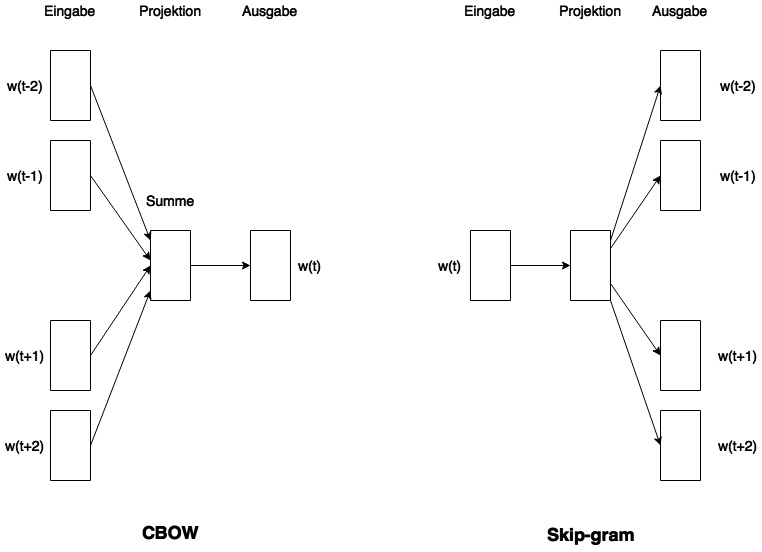
\includegraphics[scale=0.55]{CBOWvsSkip-gram.png}
  \end{center}  
  \caption{CBOW und Skip-gram im Vergleich, übersetzt nach \cite{DBLP:journals/corr/abs-1301-3781}}
  \label{cbowvsskipgram}
\end{figure}

	\section{Parameter}
	\label{sec:Parameter}
	\textbf{size}
	\vspace{1em}\\
	Mit dem Parameter \textit{size} wird die Anzahl der Dimensionen der Wortvektoren eingestellt. In einem n-Dimensionalen Vektorraum nimmt n den Wert von \textit{size} an.\\	
	\vspace{1em}\\
	\textbf{window}
	\vspace{1em}\\
	\textit{window} ist der maximale Abstand zwischen benachbarten Worten, innerhalb eines Satzes, die zur Berechnung der Wordvektoren betrachtet werden.\\
	\vspace{1em}\\
	\textbf{min\_count}
	\vspace{1em}\\
	Der Parameter \textit{min\_count} gibt an, wie oft ein Wort in den Testdaten mindestens vorkommen muss, um in das Wörterbuch aufgenommen zu werden.\\
	\vspace{1em}\\
	\textbf{negative}
	\vspace{1em}\\
	Dieser Parameter wird nur benötigt, wenn als Lernalgorithmus negative sampling verwendet wird\footnote{siehe \ref{sec:negativeSampling} Negative sampling}. Er gibt an, wie viele zufällig ausgewählten Worte verwendet werden sollen.
	
	\section{CBOW}
	CBOW ist die Abkürzung für Continuous bag-of-words (dt. stetige Menge an Worten). Beim CBOW wird ein neuronales Netz ohne verdeckte Schichten (hidden layer) verwendet\cite{DBLP:journals/corr/abs-1301-3781}.\\
	In der CBOW Architektur wird aus dem Kontext ein Wort vorhergesagt (siehe Abbildung \ref{cbowvsskipgram}). Die Anzahl, der aus dem Kontext zu verwendende Worte, wird mit dem Parameter \textit{window} angegeben.
	
	\section{Skip-gram}
	Bei der Skip-gram Architektur wird auch, wie beim CBOW Model, ein neuronales Netz ohne verdeckte Schichten (hidden layer) verwendet \citep{DBLP:journals/corr/abs-1301-3781}.\\
	Allerdings wird hier nicht ein Wort aus dem Kontext vorhergesagt, sondern aus einem Wort wird der Kontext vorhergesagt (siehe Abbildung \ref{cbowvsskipgram}).\\
	
	Mehrere verdeckte Schichten in neuronalen Netzen machen die Modelle genauer, allerdings kommt auch die meiste Komplexität des ganzen Models von solchen verdeckten Schichten \citep{DBLP:journals/corr/abs-1301-3781}. Mikolov et al. haben deshalb neuronale Netze ohne verdeckte Schichten bevorzugt, da damit sehr große Datenmengen viel effizienter gelernt werden können.
	
	\section{Hierarchical softmax}
	Eine Annäherung an das allgemeine softmax ist das hierarchical softmax \citep{DBLP:journals/corr/MikolovSCCD13}. Der Hauptvorteil ist, dass anstatt W Ausgabeknoten im neuronalen Netz nur ungefähr $log_2(W) $ Knoten ausgewertet werden müssen um die Wahrscheinlichkeiten zu errechnen. \\
	Bei diesem Lernalgorithmus wird das Wörterbuch als Huffman Binärbaum dargestellt. Dies hat den weiteren Vorteil, dass häufig genutzte Worte kurze Kodierungen haben, was sich auf das Trainingstempo positiv auswirkt.
	
	\section{Negative sampling}
	\label{sec:negativeSampling}
	Alternativ zum hierarchical softmax kann das negative sampling als Lernalgorithmus für das neuronale Netz verwendet werden \citep{DBLP:journals/corr/MikolovSCCD13}.\\
	Das negative sampling unterscheidet sich zum hierarchical softmax insofern, dass nicht die Ähnlichkeiten zu anderen Worten berechnet werden, sondern es wird davon ausgegangen, dass zufällig ausgewählte Worte mit einer hohen Wahrscheinlichkeit unähnlich, dem zu testenden Wort, sind. Wie viele solcher zufällig ausgewählter Worte benutzt werden sollen kann mit dem Parameter \textit{negative} angegeben werden.
	

	
	
\newpage
\chapter{Wikipedia-Korpus}
Im Folgenden Kapitel werden die in der Arbeit verwendeten Korpora erläutert und die im Word2Vec Modell benutzten Parameter begründet.\\
Des weiteren werden die benutzten Testdaten vorgestellt.
\iffalse
	Kompletter Wikikorpus: \\
	8392453 Artikel\\
	wordcount: 2919802692\\
	sentencecount: 242144317\\
	
	
	Techkorpus:\\
	187144 Artikel (2,2%)\\
	wordcount: 9866096 (0,34%)\\
	sentencecount: 3166065 (1,3%)\\
\fi
	\section{Gesamtkorpus}
	\label{sec:Gesamtkorpus}
	Da sich die Qualität  der Wortvektoren im Word2Vec Modell wesentlich mit der Menge an Trainingsdaten erhöht\citep{DBLP:journals/corr/abs-1301-3781}, werden möglichst große Textkorpora bevorzugt. Auf der Google Code Seite von Word2Vec\footnote{https://code.google.com/p/word2vec/, abgerufen am 29.06.2015}, werden für Forschungszwecke einige Beispiele für online verfügbare große Korpora genannt. Unter anderem auch der neueste Wikipedia Auszug\footnote{http://dumps.wikimedia.org/enwiki/latest/enwiki-latest-pages-articles.xml.bz2, abgerufen am 29.06.2015}.\\
	Da in dieser Arbeit ein allgemeiner und ein domänenspezifischer Korpus als Trainingsdaten für das Word2Vec Modell verglichen werden sollen, eignet sich der Wikipedia Korpus gut. \\
	Wie in \ref{sec:Vorverarbeitung} beschrieben, müssen die Daten erst einer Säuberung unterzogen werden um dann anschließend im Word2Vec Modell trainiert zu werden.\\
	 Der bereinigte, komplette englischsprachige Wikipedia Korpus\footnote{Dump von März 2015, http://dumps.wikimedia.org/enwiki/latest/enwiki-latest-pages-articles.xml.bz2, abgerufen am 09.04.2015} enthält 8.392.453 Artikel, 242.144.317 Sätze und 2.919.802.692 Worte.\\


Die Skip-gram Architektur verhält sich im Bezug auf syntaktische Ähnlichkeit etwas schlechter als die CBOW Architektur, allerdings ist die Skip-gram Architektur im Bezug auf semantische Ähnlichkeit der CBOW weit überlegen\citep{DBLP:journals/corr/abs-1301-3781}.\\ Aus diesem Grund wurde die Skip-gram Architektur ausgewählt.\\
Da der \textit{hierarchical softmax} Lernalgorithmus eher für selten vorkommende Worte und der \textit{negative sampling} Lernalgorithmus eher für häufig vorkommende Worte und niedrigdimensionale Vektoren geeignet ist\footnote{https://code.google.com/p/word2vec/\#Performance, abgerufen am 01.07.2015}, fiel die Wahl auf den \textit{hierarchical softmax} Lernalgorithmus, da das Modell (wie im Folgenden gezeigt) eine hohe Dimension der Vektoren hat und auf technologiespezifische Daten getestet werden soll (siehe \ref{sec:Testdaten} Testdaten).\\


Um die optimalen Parameter für das Training des Modells herauszufinden wurde ein kleinerer Wikipedia Auszug\footnote{http://mattmahoney.net/dc/enwik9.zip, abgerufen am 30.06.2015, beinhaltet die ersten 1 Milliarde Zeichen des Gesamtkorpus} benutzt und mit den unterschiedlichen Parametern\footnote{Siehe \ref{sec:Parameter}. Auf der Google Code Seite von Word2Vec wird eine window size bei der Skip-gram Architektur von um die 10 vorgeschlagen.} gelernt und evaluiert (siehe Tabelle \ref{tab:VergleichParameter}).\\
Die Word2Vec-Klasse in der Gensim-Implementierung beinhaltet eine Evaluationsfunktion\footnote{\textit{gensim.models.word2vec.Word2Vec.accuracy(FILENAME)}}, die die Accuracy des Models berechnet. Die Funktion erwartet einen Dateinamen einer Datei, in der jede Zeile ein 4-Tupel ist und die einzelnen Abschnitte mit \glqq : SECTION NAME\grqq{} unterteilt sind. Auf der Google Code Seite ist eine solche Datei als Beispiel vorhanden\footnote{https://code.google.com/p/word2vec/source/browse/trunk/questions-words.txt, abgerufen am 29.06.2015}. In diesem Beispiel sind 14 Kategorien\footnote{\textit{capital-common-countries, capital-world, currency, city-in-state, family, gram1-adjective-to-adverb, gram2-opposite, gram3-comparative, gram4-superlative, gram5-present-participle, gram6-nationality-adjective, gram7-past-tense, gram8-plural, gram9-plural-verbs}} mit insgesamt 19544 4-Tupel aufgelistet.\\

\begin{table}[h]
\label{tab:VergleichParameter}
\caption{Vergleich Parameter}
\begin{center}
\begin{tabular}{l|l|l|l}\\
\textbf{Size} & \textbf{Window} & \textbf{Min\_count} & \textbf{Gesamtaccuracy}\\
\hline	
400 & 10 &  5 & 53,5\%\\
400 & 10 & 10 & 52,5\%\\
300 & 10 &  5 & 52,5\%\\
300 & 10 & 10 & 52,9\%\\
200 & 10 &  5 & 50,5\%\\
200 & 10 & 10 & 50,5\%\\
100 & 10 &  5 & 42,0\%\\
100 & 10 & 10 & 41,3\%\\

\end{tabular}
\end{center}
\end{table}

Auf dem kleineren Wikipedia Korpus erzielte das Modell mit den Parametern 
$$\\size = 400, window = 10, min\_count = 5$$
 die beste Gesamtaccuracy mit 53,5\%.\\
Diese Parameter wurden dann auch beim Gesamtmodell angewandt.\\
Die Trainingszeit beträgt bei diesen Parametern 10,5h\footnote{Leistungsdaten: PC mit 32 GB RAM, i7-3770 Quadcore bei 3,4 GHz} beim Gesamtmodell.\\
Nachdem ein kleinerer Fehler im Reiningungsskript aufgetretetn war\footnote{Unbekannte Zeichen wurden mit einem Leerzeichen ersetzt, anstatt gelöscht zu werden, somit entstanden Wortfragmente als eigene Worte.}, musste das komplette Modell nochmals gelernt werden. Hier fiel dann die Entscheidung, andere Parameter zu benutzen und die \textit{window} Größe auf 300 zu reduzieren, da die Accuracy sich nur sehr gering verändert hat, allerdings verkürzte sich die Trainingszeit auf 7,7h. Dies zahlte sich im Laufe der Arbeit aus, da sich das Perl-Reinigungsskript ein paar Mal geringfügig änderte um so kleinere Fehler aus dem Korpus zu entfernen.\\


	
	\section{Teilkorpus}
	\label{sec:Teilkorpus}	
	Der zweite Korpus ist wie in \ref{sec:Vorverarbeitung} beschrieben, ein Teilkorpus, bestehend aus Technologieartikeln des Gesamtkorpus. Dieser domänenspezifische Teilkorpus enthält 187.144 Artikel (2,2\% im Vergleich zum Gesamtkorpus), 9.866.096 Wörter(0,34\%) und 3.166.065 Sätze(1,3\%). Hier beträgt die Trainingszeit ca. 2 Minuten.\\
	Wird dieser Korpus mit der \textit{.accuracy()}-Methode evaluiert, erreicht er eine Gesamtaccuracy von nur 7,0\%. Das hat den Grund, dass die Testfragen sehr allgemeiner Art sind und diese Beziehungen in einem reinen Technologiekorpus sehr selten bis gar nicht vorkommen.\\
	
	Es wäre auch möglich gewesen, andere Daten\footnote{z.B. Foren, Technews Internetseiten o.ä.} zu benutzen. Die Wahl fiel aber auf den Teilkorpus von Wikipedia, da hier die gleichen Texte in beiden Korpora vorhanden sind und somit auch die gleichen Beziehungen zwischen den einzelnen Wörtern, um so einen möglichst objektiven Vergleich zwischen den unterschiedlichen Korpora zu ermöglichen.\\
	
	
	\section{Testdaten}
	Die Testdaten umfassen 236 Begriffe (siehe Anhang \ref{sec:Testdaten}) aus der Domäne Technologie. Die Testdaten werden dazu verwendet, um die ähnlichen Worte in den Modellen zu untersuchen und zu vergleichen. Die genauen Fragestellungen und Experimente werden im Kapitel \ref{chap:Experimente} Experimente ausführlich beschrieben.
	
	
\newpage
\chapter{Experimente}
\label{chap:Experimente}
In diesem Kapitel sollen die unterschiedlichen Korpora (Gesamtkorpus\footnote{vgl. \ref{sec:Gesamtkorpus}} und Techkorpus\footnote{vgl. \ref{sec:Teilkorpus}}) untersucht werden. Dies soll durch ausgewählte Fragestellungen realisiert werden.
\\Die Fragestellungen beziehen sich immer auf die Ergebnisse, die aus den Tastdaten\footnote{vgl. \ref{sec:Testdaten}} erhaltenen ähnlichen Worten.
\\Jedes Experiment ist in drei Teile aufgeteilt Beschreibung, Durchführung und Interpretation/Ergebnis.\\
Zum Vergleichen der ähnlichen Worte der unterschiedlichen Korpora wurde eine Datei erzeugt, in der die Testdaten und ihre fünf ähnlichsten Worte sowie deren fünf ähnlichsten Worte (Rekursion), leserlich formatiert, ausgegeben werden.\\ 

	\section{Synonymsuche durch Rekursion}
		\subsection{Beschreibung}
		Es soll untersucht werden, ob es möglich ist, Synonyme eines Begriffs zu finden, indem man die vom Modell erhaltenen ähnlichen Worte dieses Begriffs erneut als Input(Suchbegriffe) der Methode  \textit{most\_similar()} verwendet. Also durch einmalige Rekursion.\\
Eine Anwendung hierfür könnte ein Thesaurus-Lexikon sein.

		
		
		\subsection{Durchführung}
		Oft war der Suchbegriff aus den Testdaten mit in den ähnlichen Wörtern der ähnlichen Wörter. Da in diesem Experiment pro Suchbegriff 25 Ergebnisbegriffe untersucht werden mussten, nahm es etwas mehr Zeit in Anspruch als die übrigen Experimente. Zudem waren viele Begriffe sehr themenspezifisch, deren Zusammenhang mit dem Suchbegriff aus den Testdaten erst einmal herausgefunden werden musste.\\
		Im Technologiekorpus waren einige Suchbegriffe nicht enthalten.\\
		Sobald ein Synonym vorhanden war, wurde der Suchbegriff als \textit{Synonym enthalten} markiert.
	
\begin{table}[h]
\caption{Experiment 1: Synonyme durch Rekursion}
\begin{center}
\begin{tabular}{|l||l|l|l|l|}
\hline
Korpus & Synonyme & Synonyme  & Wort nicht  & Relation\\
 & nicht enthalten & enthalten & im Korpus & \\

\hline
 Komplett & 187 & 49 & 0 & 20,8\% \\
 \hline
 Technologie & 191 & 20 & 25 & 8,5\% (9,5\%)\\
 \hline
 
\end{tabular}
\end{center}
\end{table}
		Die Prozentangabe in Klammern bezieht sich auf die Relation zu den im Korpus enthaltenen Worte (211 Stück) und nicht auf die Gesamtzahl an Testdaten(236 Stück).\\
		
Einige Beispiele:\\
 
\begin{table}[h]
\caption{Beispiele von Synonyme durch Rekursion}
\begin{center}
\begin{tabular}{|l||l|l|l|l|}
\hline
Suchbegriff & Korpus & Synonyme   \\

\hline
 3d & Komplett & threedimensional, stereoscopic, autostereoscopic \\
  	& Technologie& threedimensional, autostereoscopic\\
 \hline	
 bitcoin	& Komplett	& cryptocurrencies	\\
 	\hline
 hd	 & Komplett 	& 1080p, 1920x1080 \\
  	 & Technologie	& 1080p, 1920x1080 \\
 	\hline
 keyboard	& Komplett & synthesizer	\\
 	\hline
 wifi	&	Komplett &	wlan\\
 	\hline
 
\end{tabular}
\end{center}
\end{table}
		
\begin{figure}[p]
  \begin{center}
	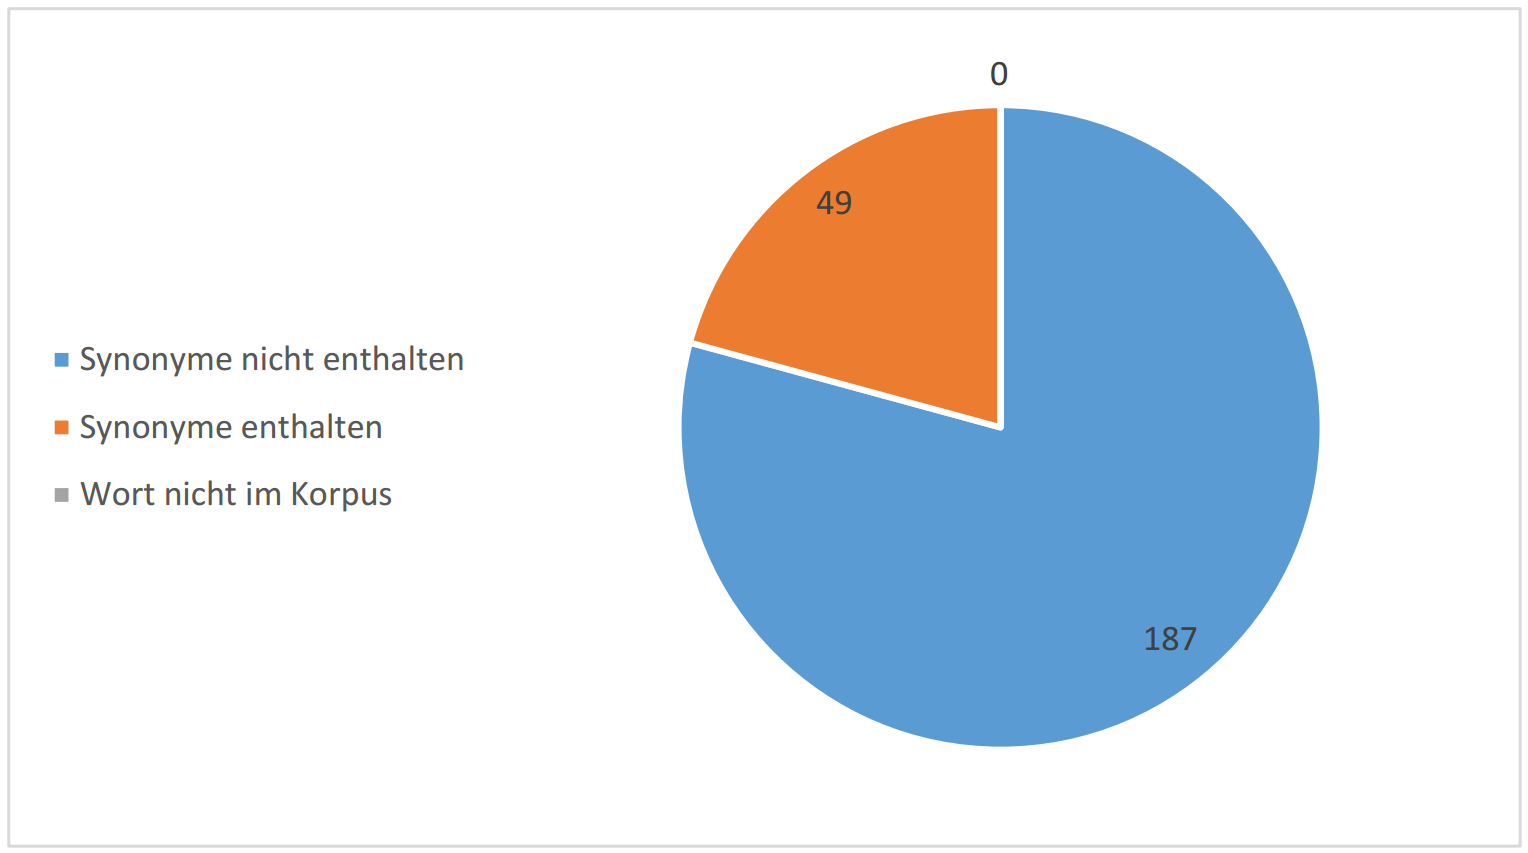
\includegraphics[scale=0.4]{SynonymFull.PNG}
  \end{center}  
  \caption{Synonyme durch Rekursion kompletter Korpus.}

\end{figure}
 

\begin{figure}[p]
  \begin{center}
	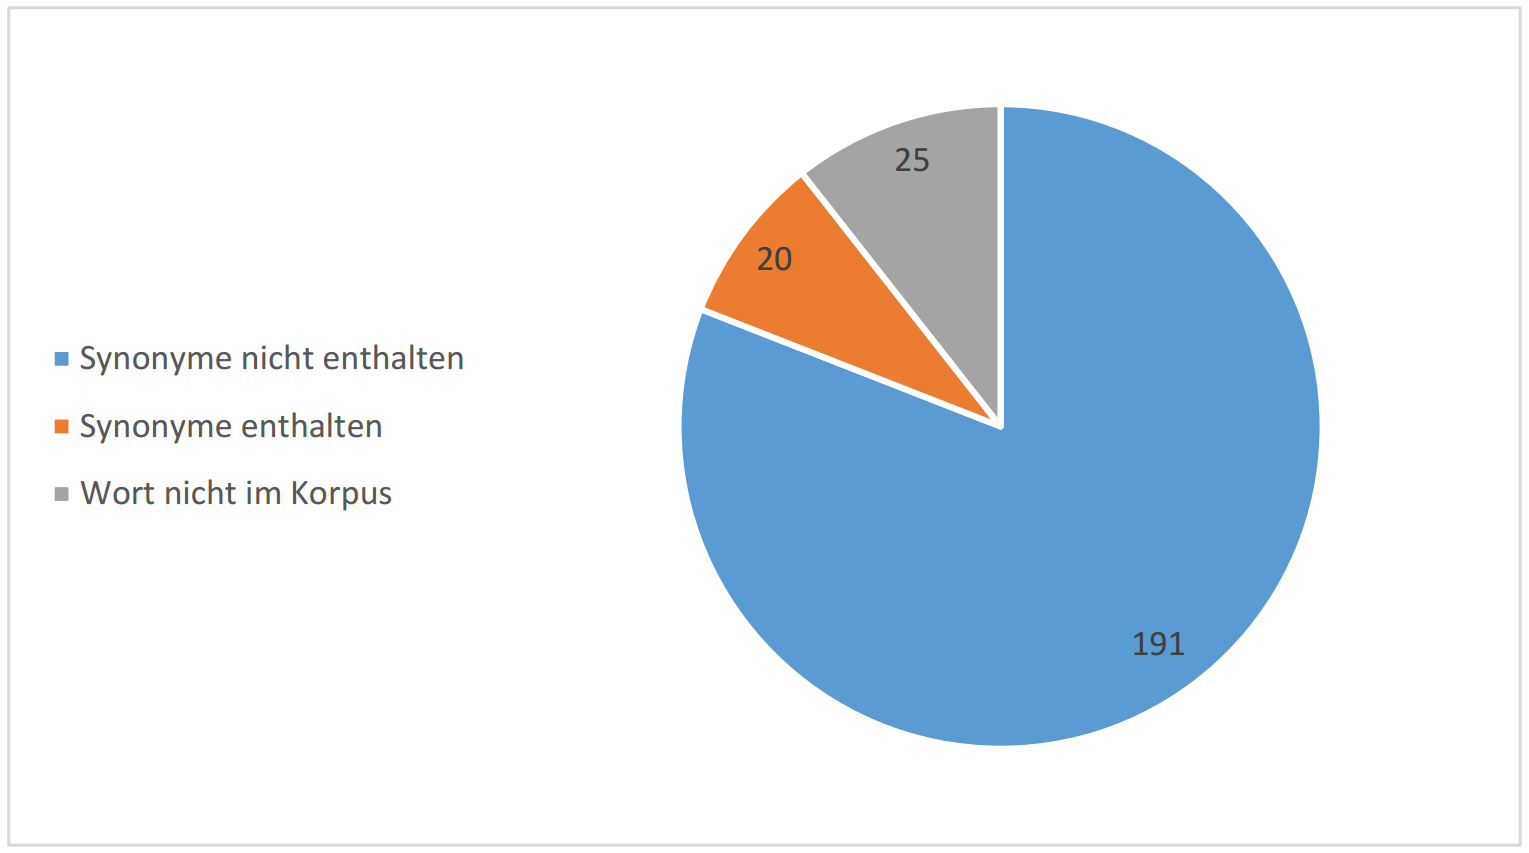
\includegraphics[scale=0.4]{SynonymTech.PNG}
  \end{center}  
  \caption{Synonyme durch Rekursion Technologiekorpus.}
  
\end{figure}
		\subsection{Interpretation/Ergebnis}
		Wie aus den Daten hervorgeht, werden zwar einige Synonyme der Suchbegriffe gefunden, allerdings nicht in großen Mengen. Dazu kommt auch, dass sich die beiden Korpora nochmal unterscheiden. Im kompletten Korpus wurden in \textit{20,8\%} der Testfälle Synonyme gefunden, wobei es im Technologiekorpus sogar nur weniger als halb so viele (\textit{8,5\%}) waren.\\
		
		Somit ist die Vermutung dieses Experiments widerlegt.
		
		
	\newpage
	\section{Konkretisierungen}
		\subsection{Beschreibung}
		In diesem Experiment ist zu untersuchen ob die ähnlichen Worte im domänenspezifischen Korpus eine Konkretisierung des Suchbegriffs darstellen.\\
		Dies ist gerade bei mehrdeutigen Worten interessant, da hier dann klar eine Definition dominant sein könnte und somit klar ist, in welchem Kontext das mehrdeutige Wort in dieser Domäne gemeint ist.\\
		\subsection{Durchführung}
		Die Fragestellung bezieht sich zwar nur auf den domänenspezifischen Korpus, allerdings wurde auch der allgemeine Korpus auf diese Fragestellung hin untersucht.\\
		Auch bei diesem Experiment nahm das Nachschlagen von mehreren ähnlichen Worten einige Zeit in Anspruch. Denn um beurteilen zu können, ob es sich um eine Konkretisierung handelt, müssen die inhaltlichen Beziehungen zwischen Suchbegriff und ähnlichen Worten klar sein. \\
		
		
\begin{table}[h]
\caption{Experiment 2: Konkretisierung}
\begin{center}
\begin{tabular}{|l||l|l|l|l|}
\hline
Korpus & ähnliche Worte & ähnliche Worte  & Wort nicht  & Relation der\\
 & nicht konkretisiert & konkretisiert & im Korpus & konkretisierten Worte\\

\hline
 Komplett & 199 & 37 & 0 & 15,7\% \\
 \hline
 Technologie & 146 & 65 & 25 & 27,5\% (30,8\%)\\
 \hline
 
\end{tabular}
\end{center}
\end{table}
		Die Prozentangabe in Klammern bezieht sich auf die Relation zu den im Korpus enthaltenen Worte (211 Stück) und nicht auf die Gesamtzahl an Testdaten(236 Stück).\\
		

\begin{table}[h]
\caption{Beispiele zur Konkretisierung}
\begin{center}
\begin{tabular}{|l||l|l|l|l|}
\hline
Suchbegriff & Korpus & Konkretisierung   \\

\hline
 apple & Technologie & iphone (Kosinusähnlichkeit: 0,587),\\
 \hline
 architecture	   & Komplett & revival (0,774), neoclassical (0,677), gothic (0,667) \\
 & Technologie& armv7a (0,514), multicore (0,493), xmos (0,477) \\
\hline
 fat	& Technologie	& exfat (0,751), vfat (0,724), fat32 (0,709)	\\
 	\hline
 intel	 & Technologie& i7 (0,707), t2300 (0,702), i5 (0,666), i52450m (0,663) \\
 \hline
 photography	& Technologie& slrs(0,544), panoramic (0,543), polaroid (0,531)\\
 	\hline
 power	&	Komplett &	electricity (0,679), surgut2 (0,637), egbin (0,627) \\
 	\hline
 
\end{tabular}
\end{center}
\end{table}
		
\begin{figure}[p]
  \begin{center}
	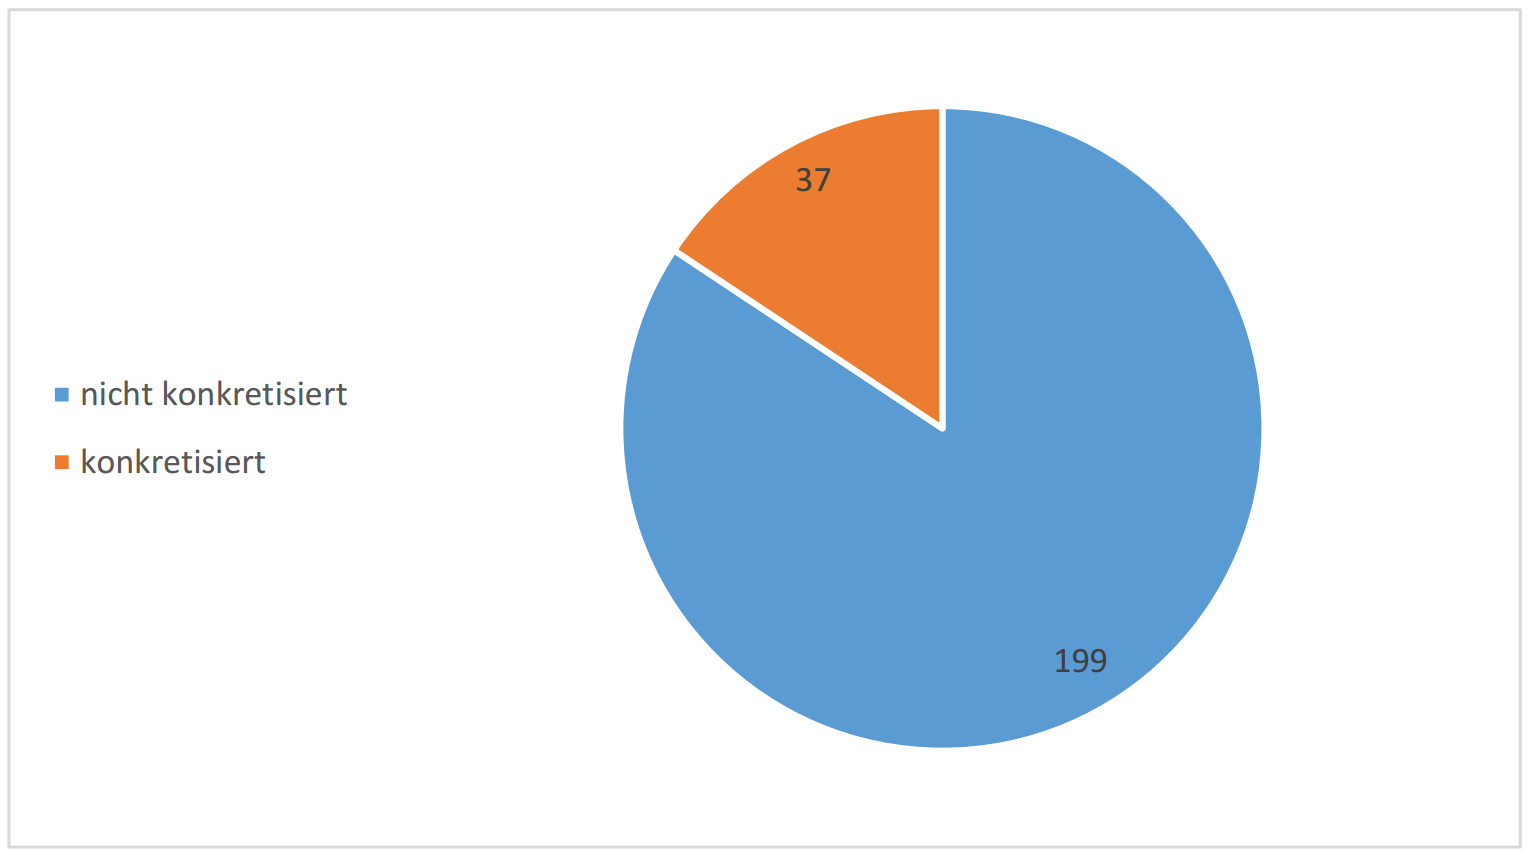
\includegraphics[scale=0.4]{KonkretisierungFull.PNG}
  \end{center}  
  \caption{Konkretisierung der Testdaten im kompletten Korpus.}

\end{figure}
\begin{figure}[p]
  \begin{center}
	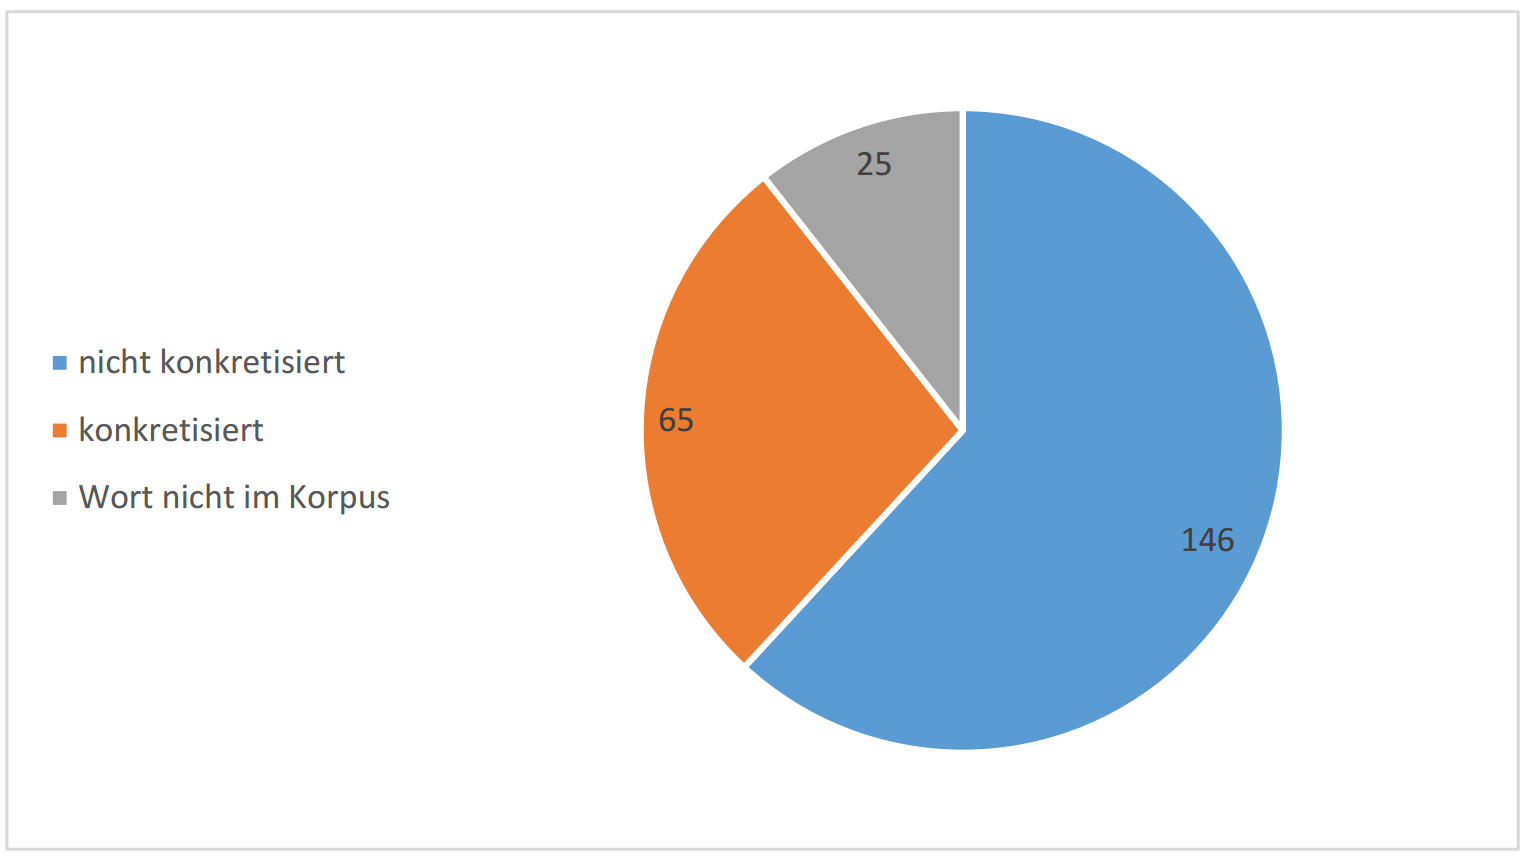
\includegraphics[scale=0.4]{KonkretisierungTech.PNG}
  \end{center}  
  \caption{Konkretisierung der Testdaten im Technologiekorpus.}
  \end{figure}	
		\newpage
		\subsection{Interpretation/Ergebnis}
		Zu beobachten ist, dass der Technologiekorpus besser konkretisiert, als der komplette allgemeine Korpus. Da dies aber nur in ca. 30\% der Testfälle passiert, ist es schwierig, zu verallgemeinern, dass die ähnlichen Worte im Technologiekorpus eine Konkretisierung sind, somit ist auch hier die Annahme des Experiments widerlegt.
		
		
	\newpage
	\section{Verallgemeinerungen}
		\subsection{Beschreibung}
		In diesem Experiment soll untersucht werden, ob die ähnlichen Worte im allgemeinen kompletten Korpus eine Verallgemeinerung des Suchbegriffs darstellen.\\
		
		\subsection{Durchführung}
		Die Fragestellung bezieht sich zwar nur auf den allgemeinen Korpus, allerdings wurde auch der Technologiekorpus auf diese Fragestellung hin untersucht.\\
		Wie beim vorherigen Experiment mussten viele Begriffe nachgeschlagen werden,  um die inhaltlichen Beziehungen zwischen Suchbegriff und ähnlichen Worten beurteilen zu können.\\
		
\begin{table}[h]
\caption{Experiment 3: Verallgemeinerung}
\begin{center}
\begin{tabular}{|l||l|l|l|l|}
\hline
Korpus & ähnliche Worte & ähnliche Worte  & Wort nicht  & Relation der\\
 & nicht verallgemeinert & verallgemeinert & im Korpus & verallgemeinerten Worte\\

\hline
\hline
 Komplett & 102 & 134 & 0 & 56,8\% \\
 \hline
 Technologie & 144 & 67 & 25 & 28,4\% (31,8\%)\\
 \hline
 
\end{tabular}
\end{center}
\end{table}

		Die Prozentangabe in Klammern bezieht sich auf die Relation zu den im Korpus enthaltenen Worte (211 Stück) und nicht auf die Gesamtzahl an Testdaten(236 Stück).\\
		
		
\begin{table}[h]
\caption{Beispiele zur Verallgemeinerung}
\begin{center}
\begin{tabular}{|l||l|l|l|l|}
\hline
Suchbegriff & Korpus & Verallgemeinerung   \\
\hline
\hline
 apple & Komplett & blackberry (Kosinusähnlichkeit: 0,704),\\
 	&	& raspberry (0,657), webos (0,643)\\
 \hline
 asus	   & Komplett & netbook (0,767), lenovo (0,736), motherboards (0,714) \\
\hline
 cookies	& Komplett& baked (0,666), cakes (0,663), sandwiches (0,655),\\
 & & muffins (0,654)	\\
 	\hline
 dell	 & Komplett & hewlettpackard (0,583), cisco (0,548), lenovo (0,515),\\
 && compaq (0,506) \\
 \hline
 limewire	& Komplett& bittorrent (0,703), filesharing (0,702), kazaa (0,689)\\
 &&rapidshare (0,668), gnutella (0,653)\\
 	\hline
 security	&	Komplett&	cybersecurity (0,702), counterterrorism (0,685), iviz (0,668) \\
 	\hline
 
\end{tabular}
\end{center}
\end{table}


\begin{figure}[p]
  \begin{center}
	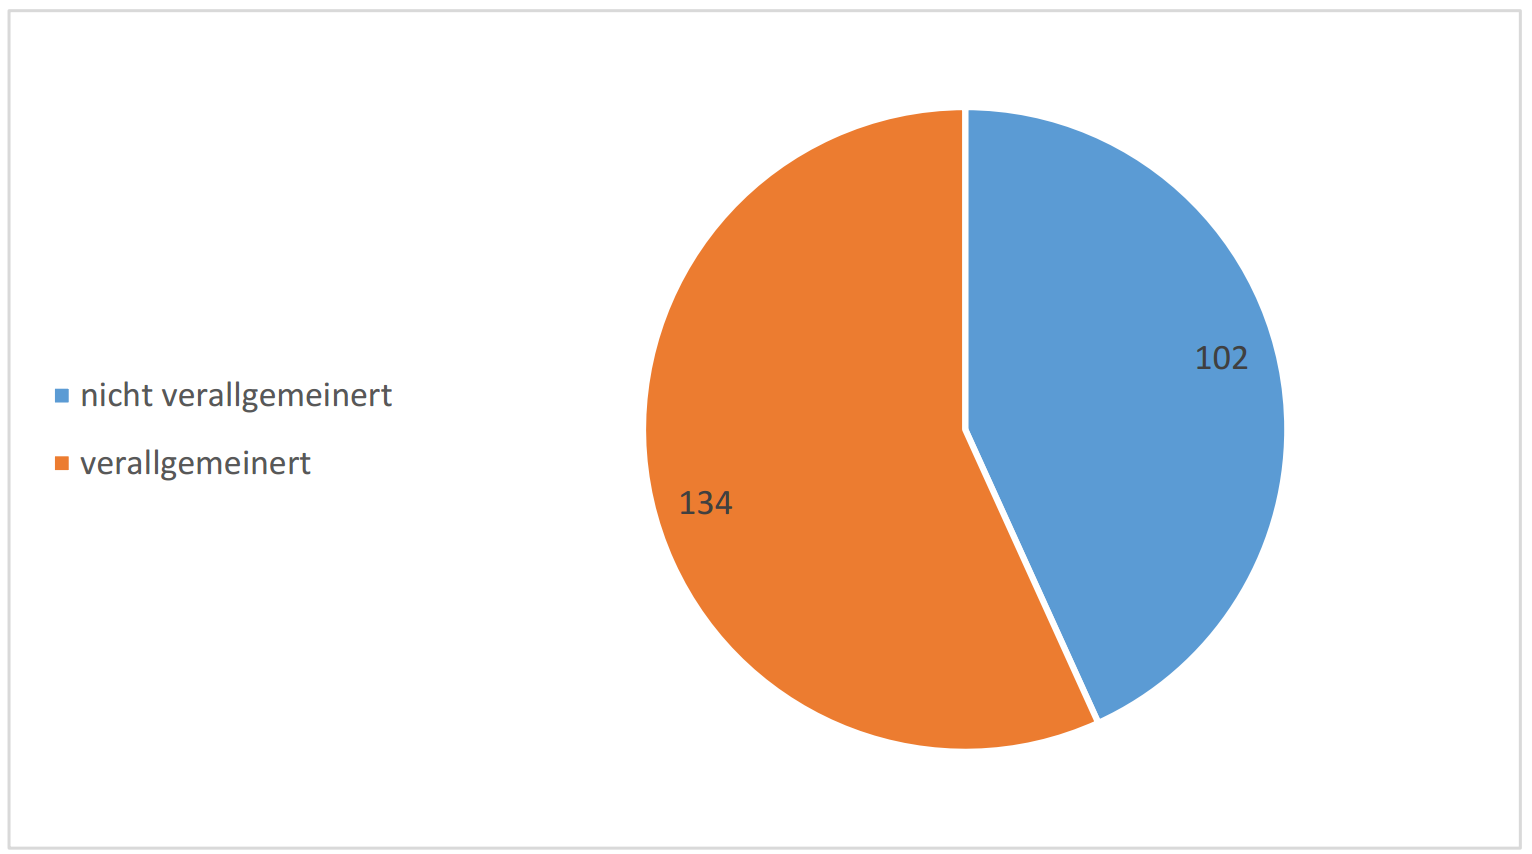
\includegraphics[scale=0.4]{VerallgemeinerungFull.PNG}
  \end{center}  
  \caption{Verallgemeinerung der Testdaten im kompletten Korpus.}

\end{figure}
\begin{figure}[p]
  \begin{center}
	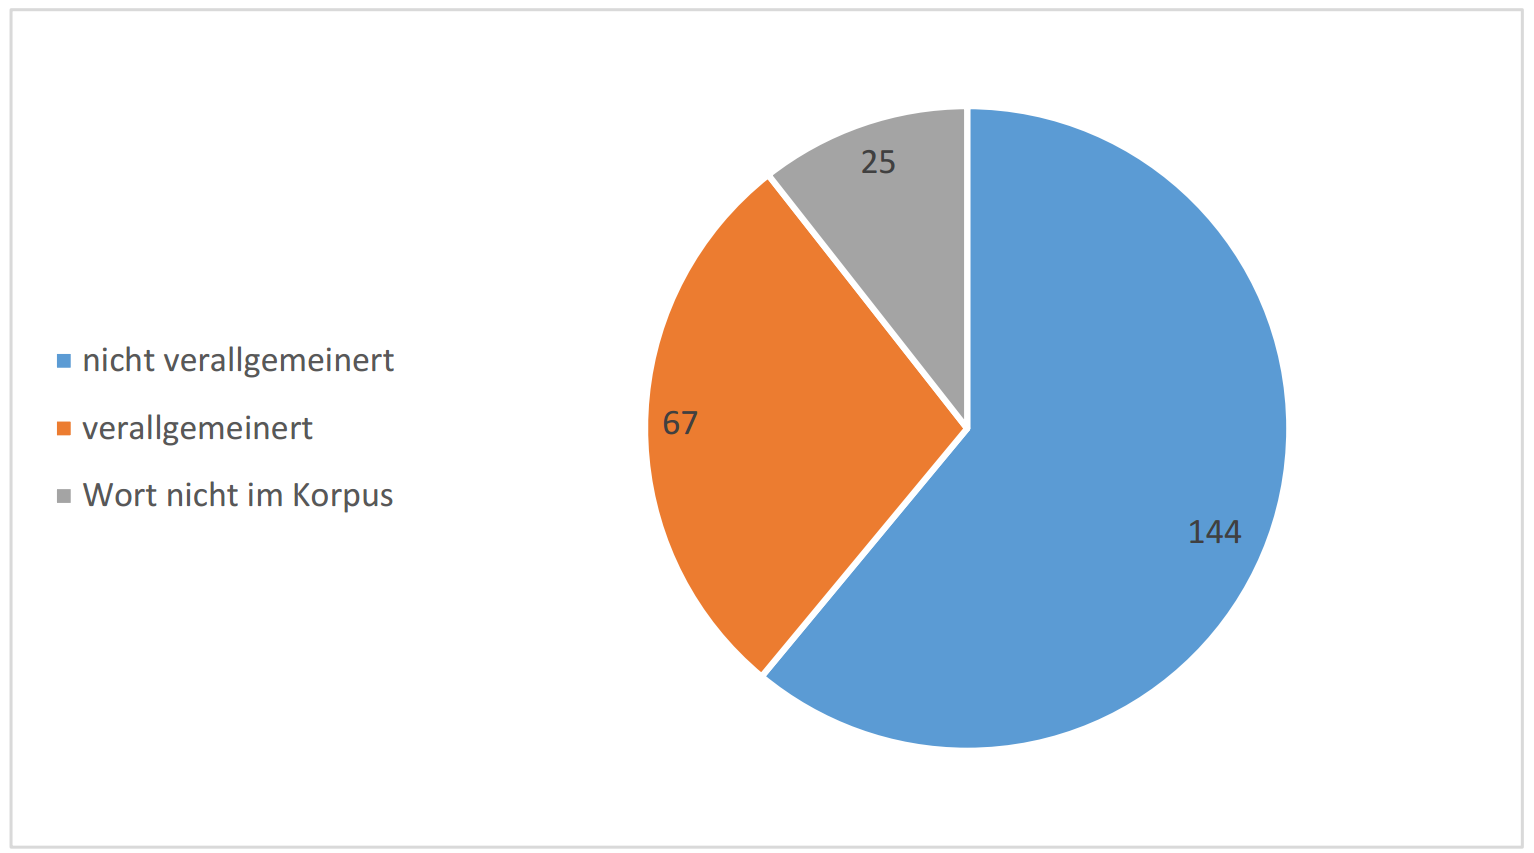
\includegraphics[scale=0.4]{VerallgemeinerungTech.PNG}
  \end{center}  
  \caption{Verallgemeinerung der Testdaten im Technologiekorpus.}
  \end{figure}	
  \newpage
		\subsection{Interpretation/Ergebnis}
		Die Untersuchungen bei diesem Experiment zeigen, dass die ähnlichen Worte eines Suchbegriffs in mehr als der Hälfte der Fälle, eine Verallgemeinerung des Suchbegriffs sind. \\
		Die Annahme dieses Experiments wurde bestätigt.\\
		
		
	\newpage
	\section{Unterschiedliche Beziehungen}
		\subsection{Beschreibung}
		In diesem Experiment soll untersucht werden, ob die Beziehungen zwischen den Suchbegriffen und den gefunden ähnlichen Worten von unterschiedlichen Arten sind. Die Beziehungen sollen in \textit{syntaktisch, synonym, gleiches, gegenteiliges, in Beziehung} und \textit{verschiedenes} eingeteilt werden.
		\subsection{Durchführung}
		Für dieses Experiment müssen beide Korpora untersucht werden, um eine Aussage machen zu können, ob sich die Beziehungsarten unterscheiden. Die Arten \textit{synonym} und \textit{gegenteilig} traten, bei den in der Arbeit verwendeten Testdaten, nicht auf. Die Art \textit{verschiedenes} wurde gewählt, wenn mehrere andere Beziehungsarten in den ähnlichen Worten vorhanden waren.
		
\begin{table}[h]
\caption{Experiment 4: Arten von Beziehungen}
\begin{center}
\begin{tabular}{|l||l|l||l|l|}
\hline
Beziehungsart	& Kompletter	& Relation & Technologie-  & Relation\\
 				& Korpus 		& 		   & Korpus		& \\

\hline
 Syntaktisch & 1 &  0,4\%	& 0 & 0,0\% \\
 \hline
 Gegenteilig & 0 & 0,0\% 	& 0 & 0,0\% \\
 \hline
 Gleiches & 81 & 34,3\% 	& 38 & 16,1\% ( 18,0\%) \\
 \hline
 Synonym & 0 & 0,0\% 	& 0 & 0,0\% \\
 \hline
 In Beziehung & 118 & 50,0\% 	& 126 & 53,4\% (59,7\%)\\
 \hline
 Verschiedenes & 36 & 15,3\% 	& 47 & 19,9\%(22,3\%) \\
 \hline
 
\end{tabular}
\end{center}
\end{table}
		
		Die Prozentangabe in Klammern bezieht sich auf die Relation zu den im Korpus enthaltenen Worte (211 Stück) und nicht auf die Gesamtzahl an Testdaten(236 Stück).\\
		

\begin{table}[h]
\caption{Beispiele zur den verschiedenen Beziehungsarten}
\begin{center}
\begin{tabular}{|l||l|l|l|l|}
\hline
Art & Suchbegriff & Korpus & Ähnliche Worte   \\
\hline
\hline
 syntaktisch&encription & Komplett & encrypted (Kosinusähnlichkeit: 0,833),\\
& 	&	& encrypts (0,798)\\
 \hline
 gleiches &chrome	   & Komplett & firefox (0,784), safari (0,686), ie8 (0,674) \\
   &	   & Technologie & firefox (0,733), safari (0,769), flock (0,667),\\
   &&& seamonkey (0,650) \\
\hline
 in Beziehung& browser	 & Komplett & browssers (0,882), firefox (0,812),\\
 &&& desktop (0,755), javascript (0,751)\\
 \hline
verschiedenes& itunes	& Komplett& spotify (0,770), beatport (0,756),\\
&&& preorder (0,718), download (0,694)\\
 	\hline
 
\end{tabular}
\end{center}
\end{table}


\begin{figure}[p]
  \begin{center}
	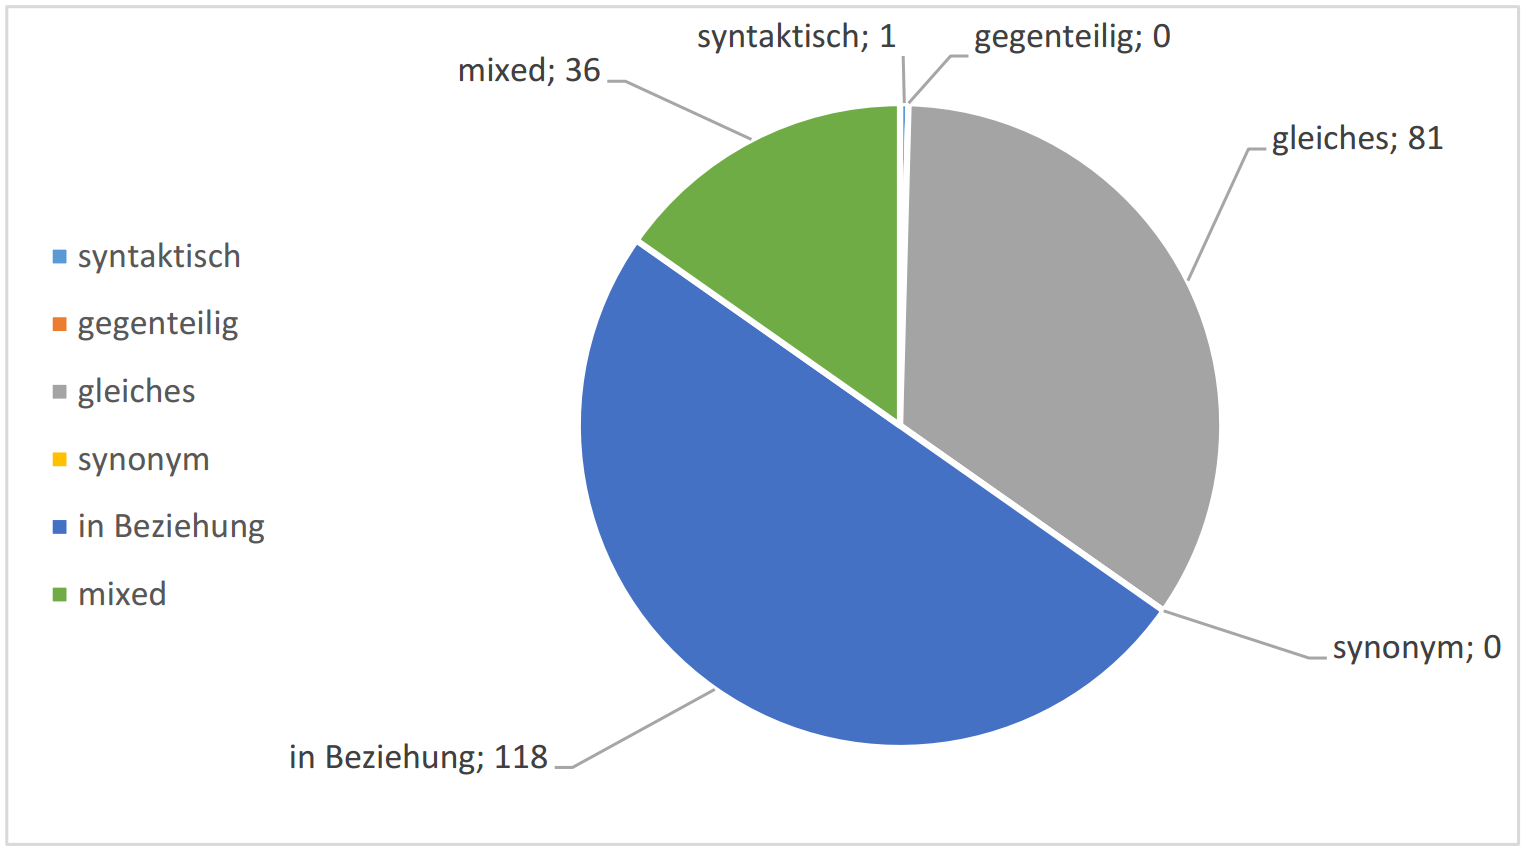
\includegraphics[scale=0.4]{BeziehungsartenFull.PNG}
  \end{center}  
  \caption{Verschiedene Arten der Beziehungen von den Testdaten zu den ähnlichen Wörtern im kompletten Korpus.}

\end{figure}
\begin{figure}[p]
  \begin{center}
	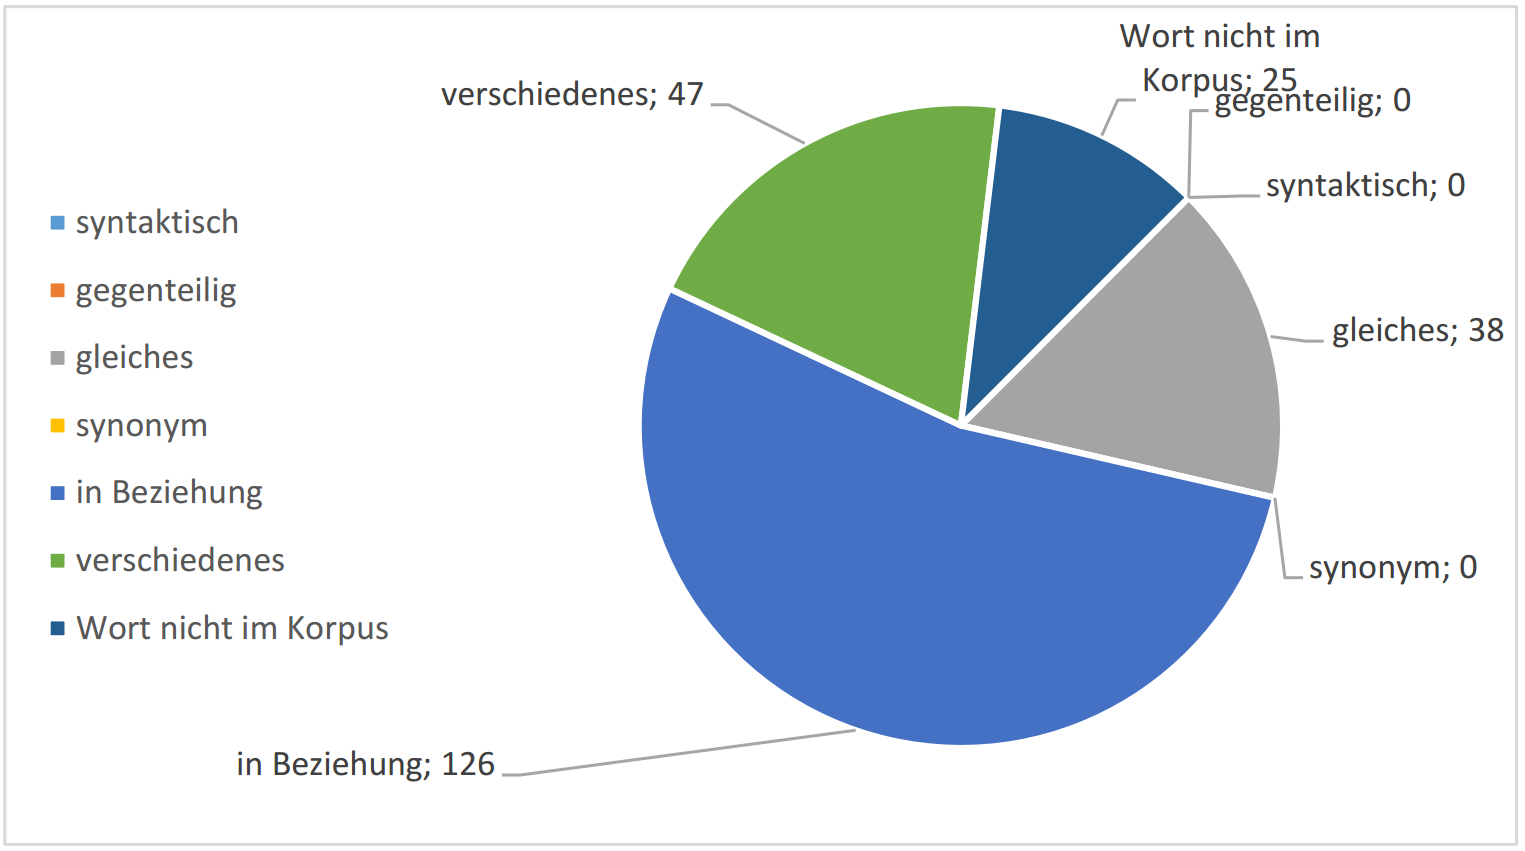
\includegraphics[scale=0.4]{BeziehungsartenTech.PNG}
  \end{center}  
  \caption{Verschiedene Arten der Beziehungen von den Testdaten zu den ähnlichen Wörtern im Technologiekorpus.}
  \end{figure}			
		
		
		
		\newpage
		\subsection{Interpretation/Ergebnis}
		Wie man in der Auswertung der Daten erkennt, ist bei beiden Korpora die Beziehungsart \textit{in Beziehung} am stärksten vorhanden, dies kommt daher, dass im Word2Vec Modell Wörter die in ähnlichem Kontext stehen, auch nahe in der Vektorrepräsentation zusammen stehen. Die Art \textit{gleiches} ist im kompletten allgemeinen Korpus mit 34,3\% die zweithäufigste Art, allerdings kommt sie im Technologiekorpus nur ca. halb so oft vor (19,9\%). Hingegen ist die Anzahl mit \textit{verschiedenen} Arten etwas höher, sowie die \textit{in Beziehung}. Der Unterschied zwischen den Beziehungsarten in den unterschiedlichen Korpora ist also nicht zu groß, allerdings deutlich erkennbar.\\
		
		
		
		
	\newpage
	\section{Erkennen von Mehrdeutigkeit}
		\subsection{Beschreibung}
		Das letzte Experiment beschäftigt sich mit der Mehrdeutigkeit von Worten. Es soll untersucht werden, ob im allgemeinen kompletten Korpus die unterschiedlichen Bedeutungen eines mehrdeutigen Wortes in den ähnlichen Worten repräsentiert werden.\\
		\subsection{Durchführung}
		Auch hier wurden beide Korpora analysiert um zu vergleichen ob sie sich unterscheiden im Bezug auf mehrdeutige Worte.\\
		
		\begin{table}[h]
\caption{Experiment 5: Erkennen von Mehrdeutigkeiten}
\begin{center}
\begin{tabular}{|l||l|l||l|l|}
\hline
				& Kompletter	& Relation 		  & Technologie-  & Relation\\
 				& Korpus 		& zur Gesamtzahl  & Korpus		& zur Gesamtzahl\\

\hline

 Wort nicht im Korpus& 0 &  0,0\%	& 24 & 10,2\% \\
 \hline
 nicht mehrdeutig & 172 &  72,9\%	& 148 & 62,7\% (70,1\%)\\
 \hline
 mehrdeutig & 64 & 27,1\% 	& 64 & 27,1\% (30,3\%)\\
 \hline 
\hline
	& Kompletter	& Relation zu	& Technologie-  & Relation zu \\
	& Korpus 		& mehrdeutigen 	& Korpus		& mehrdeutigen \\
	& 		 		& Worten	 	& 				& Worten\\

\hline
 Wort nicht im Korpus & 0 & 0,0\% 	& 1 & 1,7\%\\
 \hline
 nicht erkannt & 58 &  90,6\%	& 57 & 89,1\%\\
 \hline
 erkannt & 6 &  9,4\%	& 6 & 9,4\% \\
 \hline
\end{tabular}
\end{center}
\end{table}
		
		Die Prozentangabe in Klammern bezieht sich auf die Relation zu den im Korpus enthaltenen Worte (211 Stück) und nicht auf die Gesamtzahl an Testdaten(236 Stück).\\
		
\begin{table}[h]
\caption{Beispiele zur Erkennung von Mehrdeutigkeiten}
\begin{center}
\begin{tabular}{|l||l|l|l|l|}
\hline
Suchbegriff & Korpus & Erkannt & Ähnliche Worte   \\
\hline
\hline
 trojan & Komplett & ja &rsplug (Kosinusähnlichkeit: 0,472), athena (0,462)\\
 &	&	& bundestrojaner (0,496), centaurs (0,475), \\
 &  Technologie & ja & horse (0,586), malware (0,560), zinaps (0,476)\\
 \hline
 
raspberry& Komplett& nein & apple (0,657), apricot (0,629), \\
&&&blackcurrant (0,586),  \\
&Technologie & nein & pi (0,677), cubieboard (0,524), trimeslice (0,519)\\
\hline
 
\end{tabular}
\end{center}
\end{table}
		
		\begin{figure}[p]
  \begin{center}
	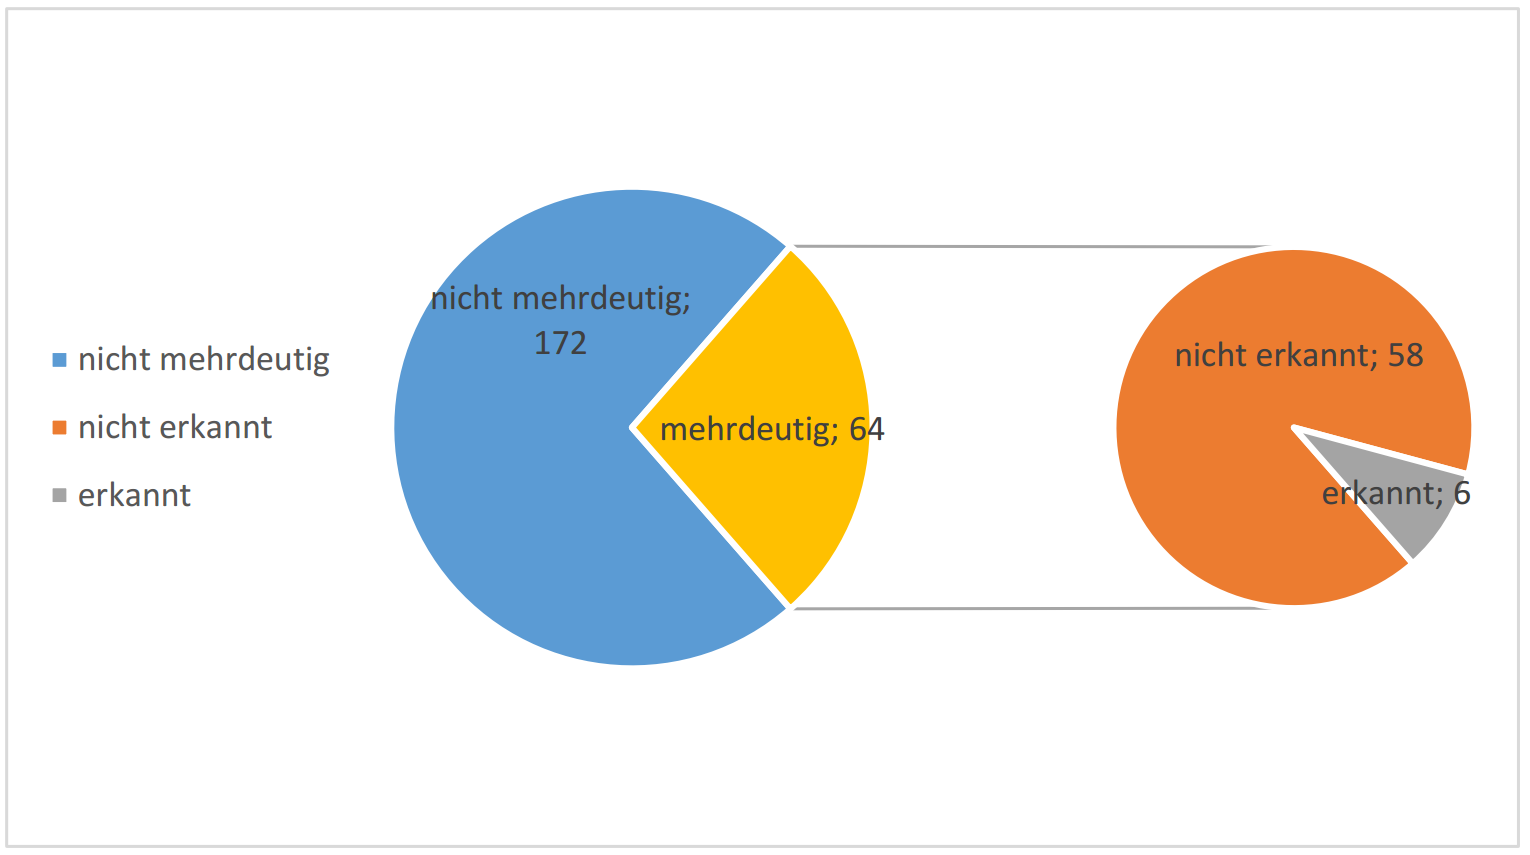
\includegraphics[scale=0.4]{MehrdeutigkeitFull.PNG}
  \end{center}  
  \caption{Erkennung von Mehrdeutigkeiten im kompletten Korpus.}

\end{figure}
\begin{figure}[p]
  \begin{center}
	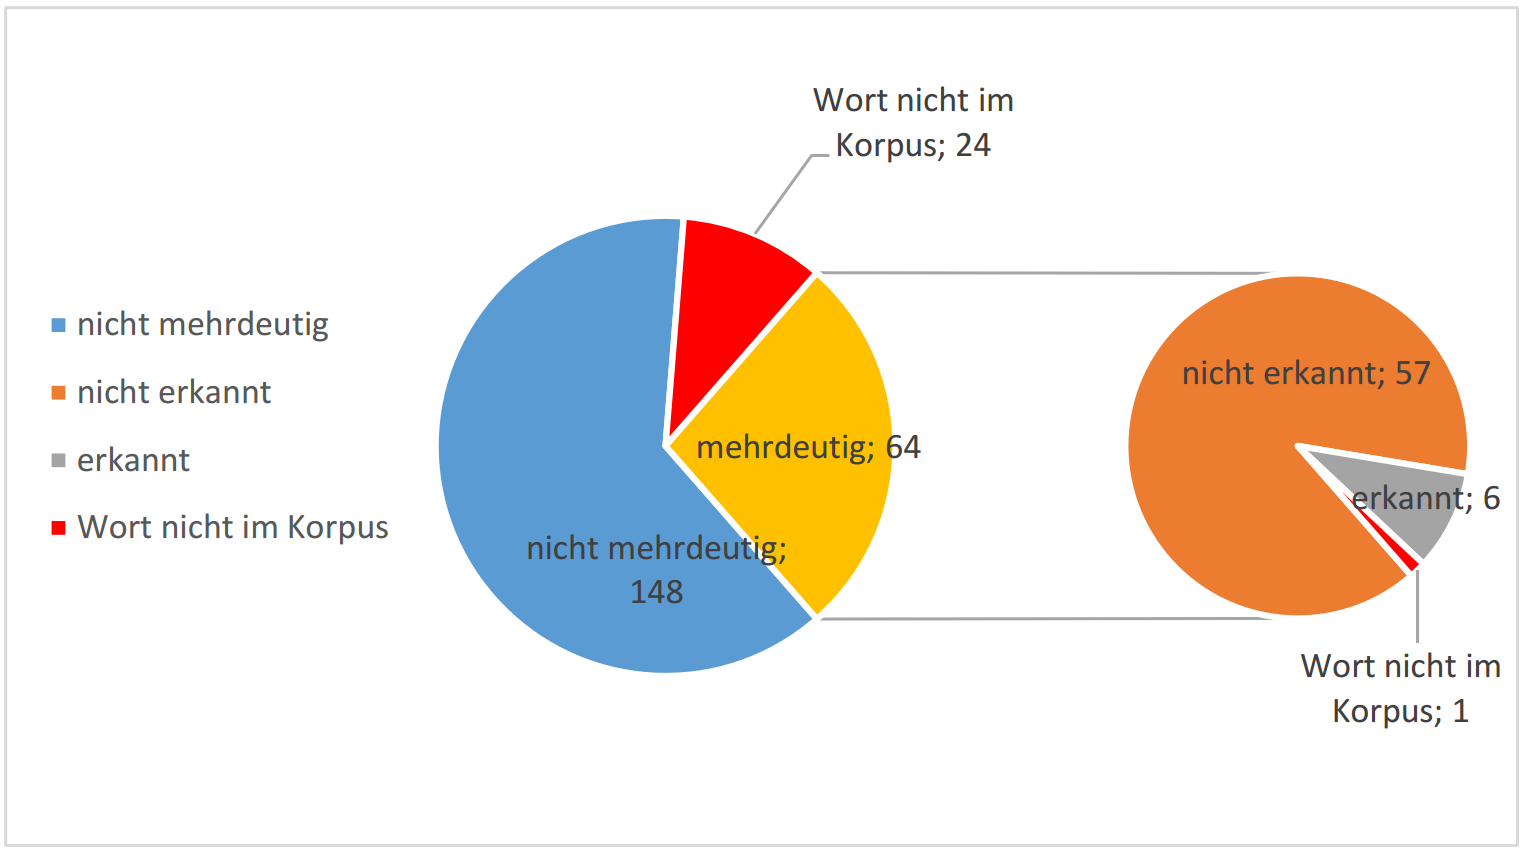
\includegraphics[scale=0.4]{MehrdeutigkeitTech.PNG}
  \end{center}  
  \caption{Erkennung von Mehrdeutigkeiten im Technologiekorpus.}
  \end{figure}	
  
		\newpage
		\subsection{Interpretation/Ergebnis}
		Erstaunlicherweise unterscheiden sich in diesem Experiment die beiden Korpora nicht in der Anzahl der erkannten Mehrdeutigkeiten. Allerdings hat öfters das eine Modell eine Bedeutung abgedeckt und das andere Modell eine oder die andere.\\
		Es ist deutlich zu erkennen, dass beide Modelle nicht geeignet sind um eine Mehrdeutigkeit in den Testdaten in ihren ähnlichen Worten abzubilden.\\
		Somit ist die Annahme dieses Experiments widerlegt.
		

\newpage
\chapter{Fazit und Ausblick}
\section{Fazit}
Nach einer ausführlichen Vorverarbeitung können die Artikel aus Wikipedia gut als Trainingsdaten für Word2Vec Modelle dienen. Dank der Gensim-Implementierung ist die Benutzung von Word2Vec sehr vereinfacht und kann komfortabel bedient werden.\\
Die Experimente liefern interessante Resultate im Bezug auf die Problemstellung zu Anfang. Durch die Experimente können die unterschiedlichen semantischen Beziehungen etwas aufgeschlüsselt werden.\\


So wird durch die Experimente klar, dass durch einmalige Rekursion der Suchbegriffe, nicht auf Synonyme des ursprünglichen Begriffs geschlossen werden kann.\\
Des weiteren eignet sich der domänenspezifische Teilkorpus eher für eine Konkretisierung der Suchbegriffe, wobei dies nur in ca. einem Drittel der Testdaten nachgewiesen werden konnte. \\
Sollen die Testdaten verallgemeinert werden, eignet sich der allgemeine komplette Korpus viel besser als der domänenspezifische Teilkorpus. Soll also ein Überblick über ein gewisses Thema oder Suchbegriff erhalten werden, wird empfohlen das Modell, welches auf dem allgemeinen kompletten Korpus trainiert wurde, zu verwenden.\\
Die unterschiedlichen Arten von Beziehung zwischen den Testdaten und ihren ähnlichen Wörtern unterscheiden sich nicht grundlegend zwischen den beiden Modellen. Das allgemeine komplette Modell hat einen etwas Größeren Anteil an \textit{gleichen} Worten, hingegen hat das domänenspezifische Teilmodell einen etwas größeren Anteil an \textit{verschiedenen} und \textit{in Beziehung} stehenden Beziehungen. \textit{Synonyme} oder \textit{gegenteilige} Arten an Beziehungen sind in beiden Modellen nicht vorhanden. Und auch \textit{syntaktische} Beziehungen sind nur bei einem Testdatensatz vorhanden.\\
Soll eine Mehrdeutigkeit gefunden werden, ist die Vorgehensweise nur die ähnlichen Worte zu vergleichen und zu analysieren, nicht zielführend. Die Modelle bilden die Mehrdeutigkeit in den ähnlichen Worten nicht gut ab. Im Ausblick wird ein Vorschlag gemacht, wie die Mehrdeutigkeit eventuell besser erfasst werden könnte.\\


Zusammenfassend kann gesagt werden, dass sich das allgemeine komplette Modell dann besser eignet, wenn ein genereller Überblick über die Testdaten erhalten werden soll. Denn in diesem Modell werden die Suchbegriffe eher verallgemeinert und die ähnlichen Worte repräsentieren \textit{Gleiches} im Bezug zu den Testdaten.\\
Soll aber ein Suchbegriff genauer untersucht, bzw. sehr fokussiert betrachtet werden, eignet sich ein domänenspezifisches Modell besser. Es konkretisiert die Testdaten nicht nur besser, sondern liefert auch fachspezifischere ähnliche Worte.\\

Die Qualität der Beziehungen hängt auch stark von den verwendeten Trainingsdaten ab. Es sollte gewährleistet sein, dass ausreichend viele und auch qualitativ gute Daten zum Training verwendet werden.\\
Soll ein domänenspezifisches Modell erstellt werden, sollte hier auch darauf geachtet werden, dass nicht nur ein Teil dieser Domäne in den Trainingsdaten abgebildet ist, außer es soll nur dieser spezielle Teil der Domäne im Modell dargestellt werden.\\


\section{Ausblick}

In der vorangegangenen Arbeit wurden einige Beziehungen zwischen den Testdaten und ihren ähnlichen Worten analysiert. In weiterführenden Arbeiten wäre es möglich, weitere und andersartige Beziehungen zwischen den Wörtern zu untersuchen. Also einfach noch mehrere Experimente durchzuführen.\\
Zum Beispiel könnte die Mehrdeutigkeit noch anders untersucht werden, indem man mehrere unterschiedliche Modelle hat und dann die ähnlichen Worte eines gleichen Testwortes vergleicht.\\

Auch könnte analysiert werden wie sich subsampling\footnote{Beim subsampling wird das Ungleichgewicht von sehr häufig und sehr selten vorkommenden Worten im Trainingskorpus verringert\citep{DBLP:journals/corr/MikolovSCCD13}. } im Word2Vec Modell, im Blick auf die in dieser Arbeit analysierten Fragestellungen, verhält.\\
Es wäre auch möglich das Word2Vec Modell mit N-Grammen, auch Phrases genannt, zu lernen, dann könnten auch Mehrwortbegriffe abgebildet und gesucht werden.





\newpage
%\chapter*{Quellenverzeichnis}
\bibliographystyle{alpha}
\bibliography{bibtex_gensim}
%\nocite{DBLP:journals/corr/abs-1301-3781}
%\nocite{DBLP:journals/corr/MikolovSCCD13}

\listoftables
\listoffigures 




\chapter{Anhang}
	\section{Testdaten}
	\label{sec:Testdaten}
\begin{table}[ht]
\caption{Testdaten Teil 1}
\begin{tabular}{l|l|l|l}\\
3d & 3ds & 3g & 4chan\\
4g & acer & acta & activision\\
adobe & amazon & android & anonymous\\
aol & apple & app & augmented\\
arcade & architecture & arpanet & asus\\
auto & automobile & battlefield & bing\\
biometrics & bitcoin & bittorrent & blackberry\\
blizzard & blogging & blog & bluray\\
broadband & browser & casual & chatroulette\\
chrome & chromebook & cispa & computing\\
console & cookies & craigslist & crowdfunding\\
crowdsourcing & cryptocurrency & cybercrime & cyberwar\\
darknet & data & dell & diablo\\
doodle & dotcom & drone & dropbox\\
e3 & ebay & email & emoji\\
encryption & energy & engine & engineering\\
ereader & events & facebook & fat\\
filesharing & firefox & flickr & foursquare\\
gadget & game & gameplay & gamergate\\

\end{tabular}
\end{table}

\newpage
\begin{table}[H]
\caption{Testdaten Teil 2}
\begin{tabular}{l|l|l|l}\\
games & gaming & ghz & gmail\\
google & googlemail & gps & groupon\\
gta & hacking & halo & handheld\\
hardware & hashtag & hd & heartbleed\\
htc & html5 & i & ibm\\
icloud & ie & imac & indie\\
instagram & intel & internet & ios\\
ipad & iphone & ipod & isp\\
itunes & keyboard & kickstarter & kindle\\
kinect & laptop & lenovo & lg\\
limewire & link & linkedin & linux\\
live & machinima & macintosh & macworld\\
malware & mario & megaupload & microsoft\\
minecraft & mmorpg & mobile & monitor\\
motoring & mouse & mozilla & myspace\\
nes & net & netbook & nfs\\
nintendo & nokia & oracle & ouya\\
p2p & paypal & pc & phablet\\
phishing & photography & photoshop & pi\\
pinterest & piracy & pirate & platform\\
playback & playstation & pokemon & power\\
processor & programming & ps & ps2\\
ps3 & ps4 & psp & python\\
raider & ram & raspberry & rayman\\
recommendation & reddit & retro & robot\\
rpg & rts & safari & samsung\\
search & security & seo & skype\\
smartphone & smartphones & smartwatch & smartwatches\\
software & sonic & sony & sopa\\
spam & spotify & steam & stream\\
starcraft & stuxnet & sun & surface\\
symbian & tablet & technology & technophile\\
ted & telecom & television & tetris\\
titanfall & tomb & trojan & tumblr\\
twitch & twitter & viber & vine\\
virus & warcraft & web & whatsapp\\
wheel & wifi & wii & wikipedia\\
windows & windows7 & wireless & worms\\
wow & xbox & xp & y2k\\
yahoo & youtube & zelda & zynga\\

\end{tabular}
\end{table}

\newpage
\section{Reinigungsskript}
	\label{sec:Perlskript}
Das Originalskript von Matt Mahoney kann unter http://mattmahoney.net/dc/textdata.html gefunden werden.
\begin{verbatim}


#!/usr/bin/perl

# Program to filter Wikipedia XML dumps to "clean" text consisting only 
# of lowercase letters (a-z, converted from A-Z), and spaces 
# (never consecutive).
# All other characters are converted to spaces.  Only text which normally
# appears in the web browser is displayed.  Tables are removed.  
# Image captions are
# preserved.  Links are converted to normal text.  
# Digits are spelled out.

# Written by Matt Mahoney, June 10, 2006.  This program is 
# released to the public domain.

$/=">";                     # input record separator
while (<>) {
  if (/<text /) {$text=1;}  # remove all but between <text> ... </text>
  if (/#redirect/i) {$text=0;}  # remove #REDIRECT
  if ($text) {

    # Remove any text not normally visible
    if (/<\/text>/) {$text=0;}
    s/<.*>//;               # remove xml tags
    s/&amp;/&/g;            # decode URL encoded chars
    s/&lt;/</g;
    s/&gt;/>/g;
    s/<ref[^<]*<\/ref>//g;  # remove references <ref...> ... </ref>
    s/<[^>]*>//g;           # remove xhtml tags
    s/\[http:[^] ]*/[/g;    # remove normal url, preserve visible text
    s/\|thumb//ig;          # remove images links, preserve caption
    s/\|left//ig;
    s/\|right//ig;
    s/\|\d+px//ig;
    s/\[\[image:[^\[\]]*\|//ig;
    # show categories without markup
    s/\[\[category:([^|\]]*)[^]]*\]\]/[[$1]]/ig;  
    s/\[\[[a-z\-]*:[^\]]*\]\]//g;  # remove links to other languages
    s/\[\[[^\|\]]*\|/[[/g;  # remove wiki url, preserve visible text
    s/{{[^}]*}}//g;         # remove {{icons}} and {tables}
    s/{[^}]*}//g;
    s/\[//g;                # remove [ and ]
    s/\]//g;
    s/&[^;]*;/ /g;          # remove URL encoded chars

    $_=" $_ ";
    ###### begin changed lines ######
    s/Ä/Ae/g;
    s/ä/ae/g;
    s/Ö/Oe/g;
    s/ö/oe/g;
    s/Ü/Ue/g;
    s/ü/ue/g;
    s/ß/ss/g;
    s/-//g;
    #removes everything else than this characters
    tr/0-9A-Za-z,.!?;\r\n / /csd; 
    ###### end changed lines ######
    chop;
    print $_;
  }
}
	\end{verbatim}
	
\end{document}
